\documentclass{../../slides-style}

\slidetitle{О методологиях разработки}{06.07.2023}

\begin{document}

    \begin{frame}[plain]
        \titlepage
    \end{frame}

    \section{Введение}
    
    \begin{frame}
        \frametitle{Программа и программный продукт}
        \begin{center}
            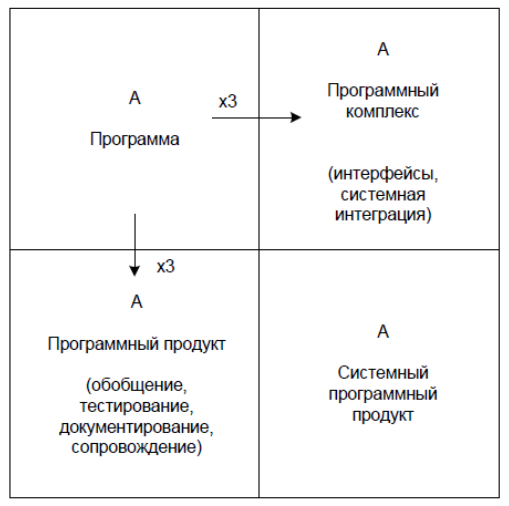
\includegraphics[width=0.5\textwidth]{mythical-man-month.png}
        \end{center}
        \begin{center}
            Ф. Брукс, ``Мифический человеко-месяц''
        \end{center}
    \end{frame}

    \begin{frame}
        \frametitle{Фазы жизненного цикла ПО}
        \begin{itemize}
            \item возникновение и исследование идеи
            \item сбор и анализ требований
            \item планирование 
            \item проектирование
            \item разработка
            \item отладка и тестирование
            \item сдача
            \item сопровождение
            \item вывод из эксплуатации
        \end{itemize}
    \end{frame}

    \begin{frame}
        \frametitle{Водопадная модель}
        \begin{center}
            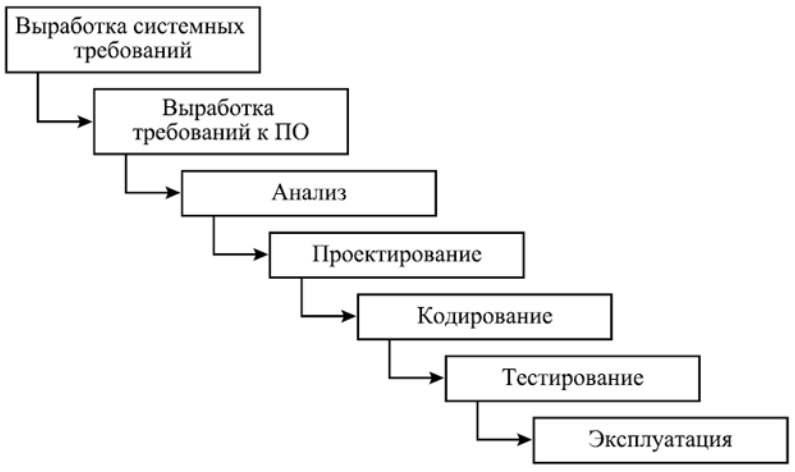
\includegraphics[width=0.7\textwidth]{waterfall-model.png}
        \end{center}
    \end{frame}

    \begin{frame}
        \frametitle{Спиральная модель}
        \begin{center}
            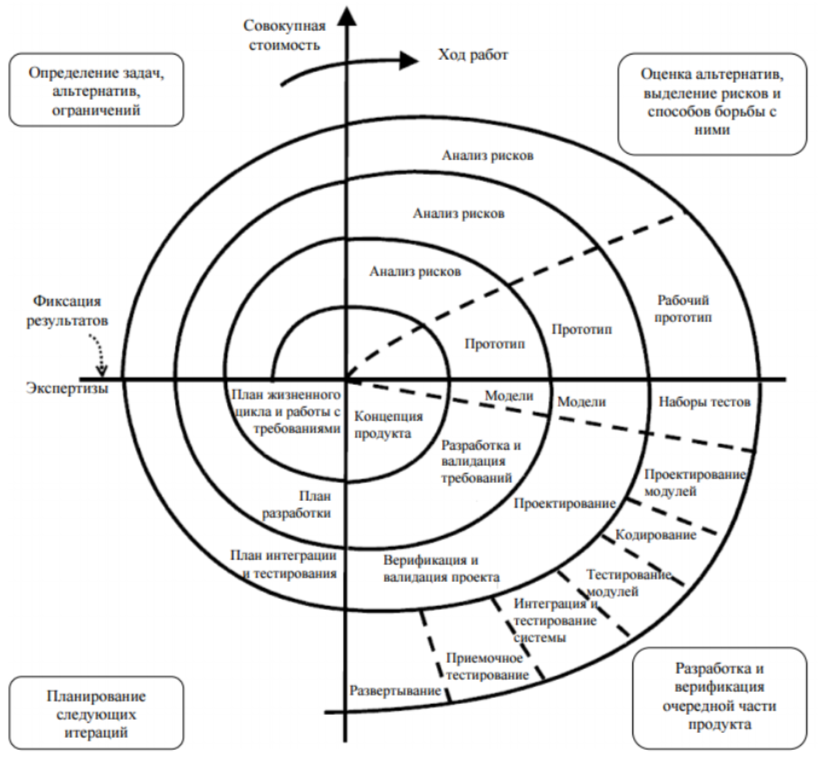
\includegraphics[width=0.6\textwidth]{spiral-model.png}
        \end{center}
    \end{frame}

    \begin{frame}
        \frametitle{Методологии разработки}
        \begin{itemize}
            \item Модели описывают последовательность фаз и что надо делать на этих фазах, методологии --- как делать
            \item ``Cowboy coding''
            \item Гибкие методологии
            \begin{itemize}
                \item Agile Manifesto
                \begin{itemize}
                    \item Люди и взаимодействие важнее процессов и инструментов
                    \item Работающий продукт важнее исчерпывающей документации
                    \item Сотрудничество с заказчиком важнее согласования условий контракта
                    \item Готовность к изменениям важнее следования первоначальному плану
                    \item Не отрицая важности того, что справа, мы всё-таки больше ценим то, что слева
                \end{itemize}
                \item XP, Scrum
            \end{itemize}
        \end{itemize}
    \end{frame}

    \begin{frame}
        \frametitle{Принципы Agile-разработки (1)}
        \begin{itemize}
            \item Наивысшим приоритетом для нас является удовлетворение потребностей заказчика, благодаря регулярной и ранней поставке ценного программного обеспечения
            \item Изменение требований приветствуется, даже на поздних стадиях разработки. Agile-процессы позволяют использовать изменения для обеспечения заказчику конкурентного преимущества
            \item Работающий продукт следует выпускать как можно чаще, с периодичностью от пары недель до пары месяцев
            \item На протяжении всего проекта разработчики и представители бизнеса должны ежедневно работать вместе
        \end{itemize}
    \end{frame}

    \begin{frame}
        \frametitle{Принципы Agile-разработки (2)}
        \begin{itemize}
            \item Над проектом должны работать мотивированные профессионалы. Чтобы работа была сделана, создайте условия, обеспечьте поддержку и полностью доверьтесь им
            \item Непосредственное общение является наиболее практичным и эффективным способом обмена информацией как с самой командой, так и внутри команды
            \item Работающий продукт --- основной показатель прогресса
            \item Инвесторы, разработчики и пользователи должны иметь возможность поддерживать постоянный ритм бесконечно. Agile помогает наладить такой устойчивый процесс разработки
        \end{itemize}
    \end{frame}

    \begin{frame}
        \frametitle{Принципы Agile-разработки (3)}
        \begin{itemize}
            \item Постоянное внимание к техническому совершенству и качеству проектирования повышает гибкость проекта
            \item Простота --- искусство минимизации лишней работы --- крайне необходима
            \item Самые лучшие требования, архитектурные и технические решения рождаются у самоорганизующихся команд
            \item Команда должна систематически анализировать возможные способы улучшения эффективности и соответственно корректировать стиль своей работы
        \end{itemize}
    \end{frame}

    \section{Scrum}

    \begin{frame}
        \frametitle{Scrum}
        \begin{itemize}
            \item На самом деле, методологический фреймворк
            \item Не акроним (на самом деле, что-то про командную работу из рэгби)
            \begin{itemize}
                \item Позволяет настраивать процесс, чем многие и злоупотребляют
            \end{itemize}
            \item Ken Schwaber/Jeff Sutherland, 1995 (на самом деле, аж в 1986 году)
            \item Инкрементальная методология со странной организацией команды, к которой никто до сих пор не может привыкнуть
        \end{itemize}
    \end{frame}

    \subsection{Роли}

    \begin{frame}
        \frametitle{Роли в команде}
        \begin{columns}
            \begin{column}{0.5\textwidth}
                \begin{itemize}
                    \item Основные 
                    \begin{itemize}
                        \item Product owner
                        \item Scrum master
                        \item Команда разработки
                    \end{itemize}
                \end{itemize}
            \end{column}
            \begin{column}{0.5\textwidth}
                \begin{itemize}
                    \item Вспомогательные 
                    \begin{itemize}
                        \item Пользователи
                        \item Заказчики
                        \item Вспомогательный менеджмент
                        \item Эксперты, консультанты
                    \end{itemize}
                \end{itemize}
            \end{column}
        \end{columns}
        \begin{center}
            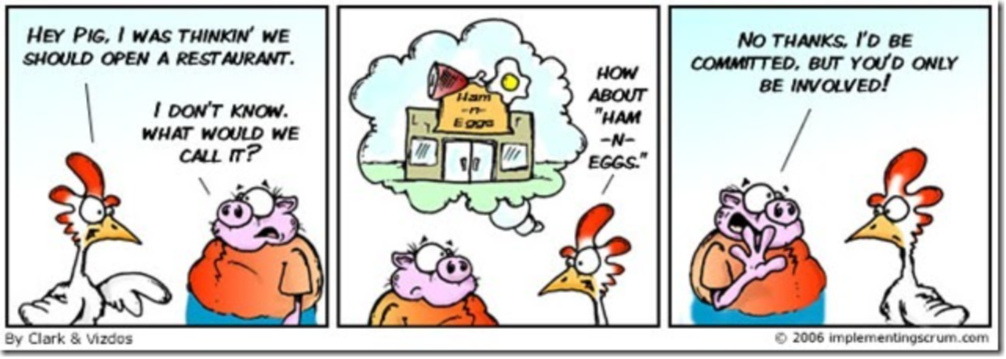
\includegraphics[width=0.8\textwidth]{ham-and-eggs.png}
        \end{center}
    \end{frame}

    \begin{frame}
        \frametitle{Product owner}
        \begin{itemize}
            \item Представляет интересы пользователей
            \begin{itemize}
                \item Его задача --- делать так, чтобы продукт был полезен
            \end{itemize}
            \item Формирует видение проекта и доносит его команде
            \item Работает с требованиями
            \item Приоритезирует задачи
            \item Отвечает за приёмку результата в конце итерации
            \item Единая точка принятия решений о задачах
            \begin{itemize}
                \item Один человек
            \end{itemize}
            \item Часть команды, работает у исполнителя
            \item НЕ начальник
        \end{itemize}
    \end{frame}

    \begin{frame}
        \frametitle{Scrum master}
        \begin{itemize}
            \item Отвечает за соблюдение методологии
            \begin{itemize}
                \item Организует митинги, организует процессы, считает метрики и т.п.
            \end{itemize}
            \item Разрешает конфликты
            \item Защищает команду от внешних факторов
            \item Помогает команде самоорганизоваться
            \item НЕ начальник
        \end{itemize}
    \end{frame}

    \begin{frame}
        \frametitle{Команда разработки}
        \begin{itemize}
            \item Те, кто, собственно, фигачат код
            \item 7 $\pm$ 2 человек
            \begin{itemize}
                \item Принцип двух пицц
                \item Должна быть очень эффективная коммуникация
            \end{itemize}
            \item Самоорганизация
            \item Кроссфункциональность
            \item Коллективная ответственность
            \item Отсутствие подкоманд
        \end{itemize}
    \end{frame}

    \subsection{Бэклог}

    \begin{frame}
        \frametitle{Product backlog}
        \begin{itemize}
            \item Список задач
            \begin{itemize}
                \item Фичи, баги, всякая вспомогательная работа (в т.ч. рефакторинги), мероприятия
            \end{itemize}
            \item Единственный источник требований
            \item Ведётся Product owner-ом
            \begin{itemize}
                \item Оценка задач выполняется командой
                \item Уточнение задачи и декомпозиция --- совместно product owner и команда
            \end{itemize}
            \item Постоянно пополняется
            \item Позиция задачи в бэклоге --- её приоритет
            \begin{itemize}
                \item Поддерживается product owner-ом
            \end{itemize}
        \end{itemize}
    \end{frame}

    \begin{frame}
        \frametitle{Пример бэклога}
        \begin{center}
            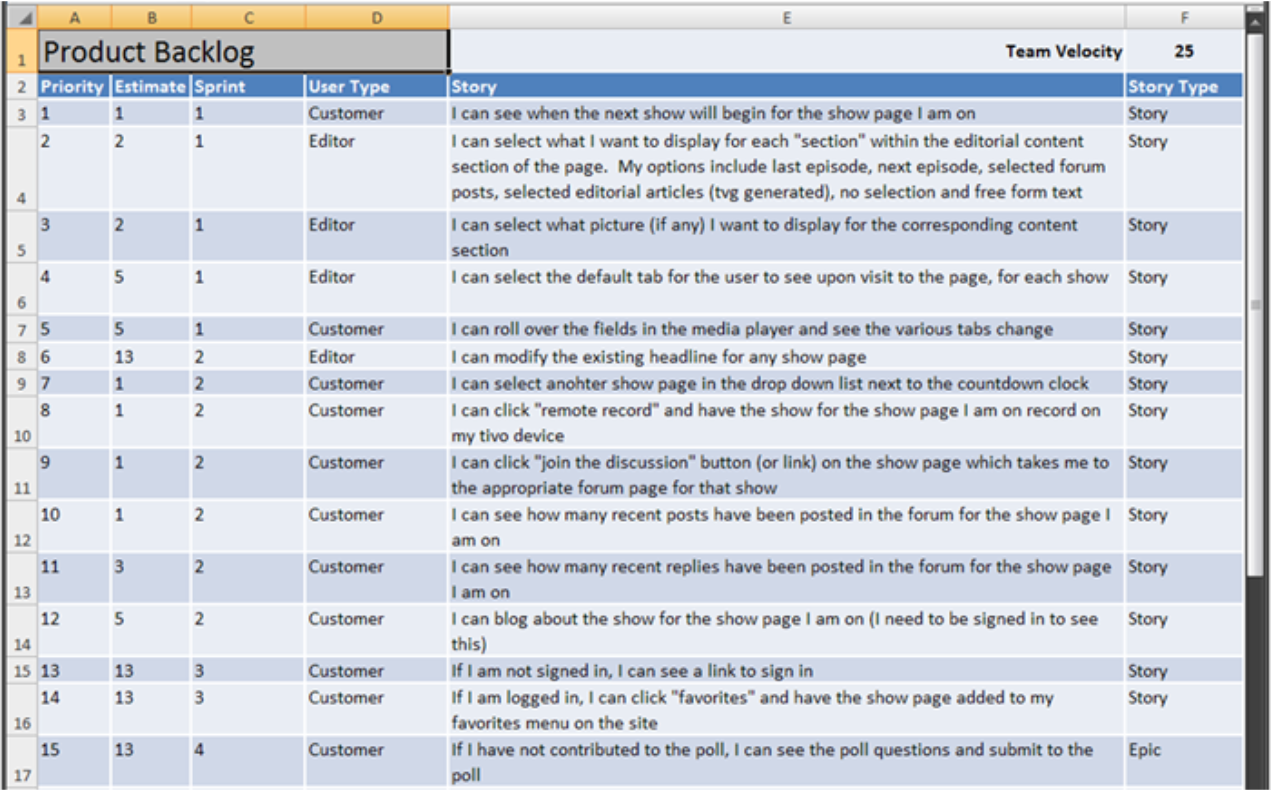
\includegraphics[width=0.8\textwidth]{backlog-1.png}
        \end{center}
    \end{frame}

    \begin{frame}
        \frametitle{Ещё пример}
        \begin{center}
            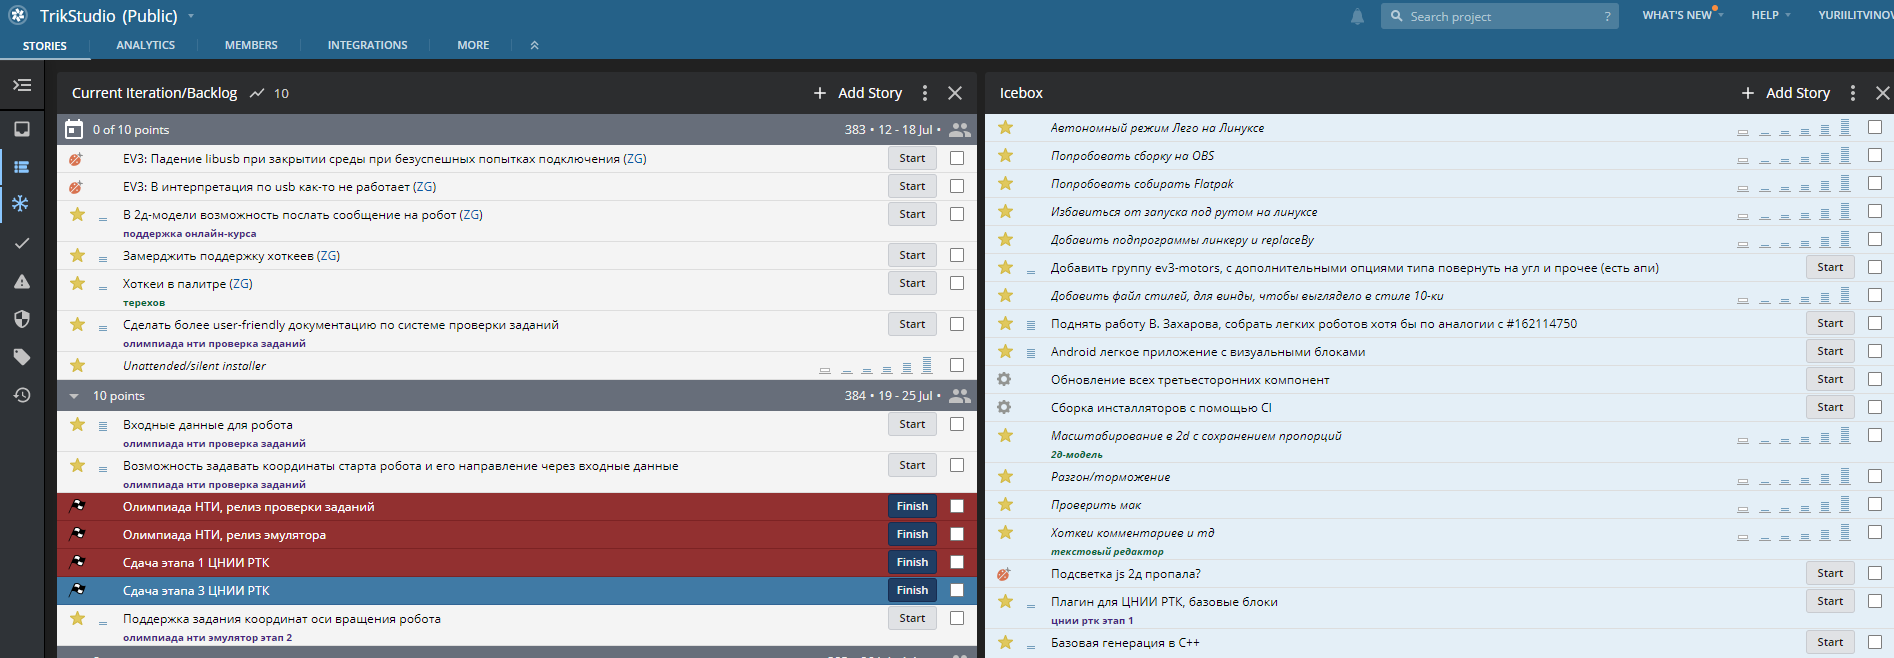
\includegraphics[width=1\textwidth]{backlog-2.png}
        \end{center}
    \end{frame}

    \subsection{Спринты}

    \begin{frame}
        \frametitle{Спринты}
        \begin{itemize}
            \item Итерация в 1-4 недели
            \item Результат --- готовая работающая версия (инкремент)
            \begin{itemize}
                \item Или хотя бы что-то осязаемое
            \end{itemize}
            \item Фиксируется объём работ, практически не меняется во время спринта
            \item Жизненный цикл:
            \begin{itemize}
                \item Планирование
                \item Разработка
                \item Демо
                \item Ретроспектива
            \end{itemize}
        \end{itemize}
    \end{frame}

    \begin{frame}
        \frametitle{Планирование}
        \begin{itemize}
            \item Обычно полдня-день в начале спринта
            \item Вся команда
            \item Определение целей спринта и набора задач
            \begin{itemize}
                \item Формируется sprint backlog
                \item Обычно просто как верхушка Product backlog, которая лезет по объёму в спринт
            \end{itemize}
            \item Оценка и упорядочивание задач
            \begin{itemize}
                \item Декомпозиция, добавление технических задач
                \item Planning poker
            \end{itemize}
            \item Коллективная оценка --- команда не знает, кто какую задачу будет делать
            \item Оценка скорости команды (team velocity)
        \end{itemize}
    \end{frame}

    \begin{frame}
        \frametitle{Planning poker}
        \begin{itemize}
            \item Условные единицы, не привязанные напрямую к линейному времени
            \begin{itemize}
                \item team velocity позволяет весьма точно пересчитать в линейный срок
            \end{itemize}
            \item Фибоначчиева шкала (1 --- сейчас сяду и сделаю, держите меня семеро; 8 --- без идей как делать)
            \item Каждый член команды выбирает свою оценку самостоятельно
            \item Потом оценки оглашаются и берётся среднее (почему и покер)
            \item Если есть сильные расхождения, задачу обсуждают, может, декомпозируют, и повторяют голосование
            \item И так по каждой задаче
        \end{itemize}
    \end{frame}

    \begin{frame}
        \frametitle{Аналоговая канбан-доска}
        \framesubtitle{Артефакт доковидной эпохи}
        \begin{center}
            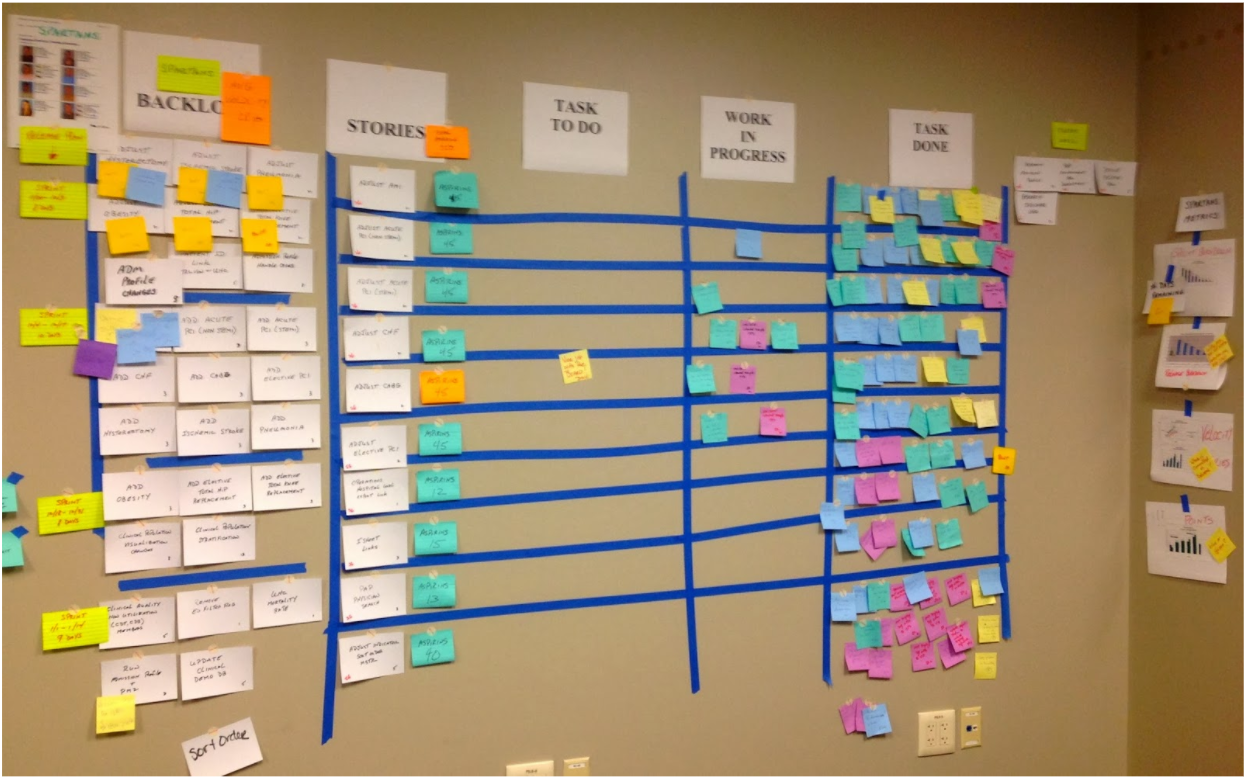
\includegraphics[width=0.95\textwidth]{kanban.png}
        \end{center}
    \end{frame}

    \begin{frame}
        \frametitle{Burndown chart}
        \framesubtitle{Burnout chart, как шутят коллеги}
        \begin{center}
            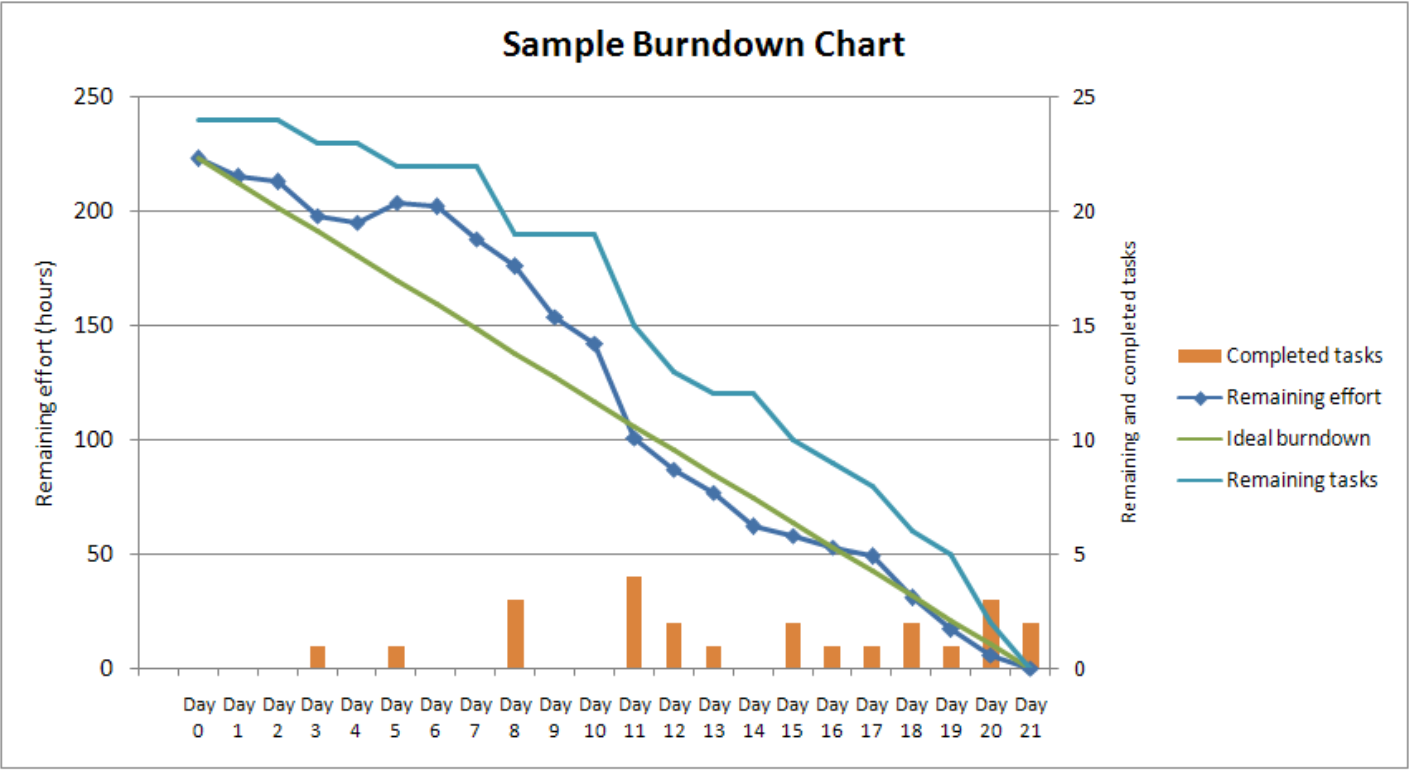
\includegraphics[width=0.95\textwidth]{burndown.png}
        \end{center}
    \end{frame}

    \begin{frame}
        \frametitle{Стэндапы}
        \framesubtitle{Они же ``daily scrum''}
        \begin{itemize}
            \item Ежедневно, не более 15 минут
            \begin{itemize}
                \item Стоя, чтобы не было желания задерживаться (опять-таки, в былые доковидные времена)
            \end{itemize}
            \item Всегда в одно время
            \item Участвуют только члены команды
            \item Что делал? Что буду делать? Какие проблемы возникли?
            \item Только делимся информацией, не решаем проблемы
            \item Если команд несколько, есть ещё скрам скрамов
        \end{itemize}
    \end{frame}

    \begin{frame}
        \frametitle{Демо}
        \framesubtitle{Оно же ``Ревью''}
        \begin{itemize}
            \item В конце спринта, не более 4 часов
            \item Демонстрация реализованного инкремента product owner-у или заказчику
            \item Приглашаются все участники проекта
            \item Проводится довольно неформально
            \item По результату обновляют backlog
        \end{itemize}
    \end{frame}

    \begin{frame}
        \frametitle{Ретроспектива}
        \framesubtitle{Чаще просто ``Ретро''}
        \begin{itemize}
            \item В конце спринта, тоже недолго (обычно демо и ретро в один день)
            \item Только команда разработки (и скрам-мастер, если он не в команде)
            \item Обсуждается процесс и всякие организационно-хозяйственные вопросы
            \begin{itemize}
                \item Что было хорошо
                \item Что можно улучшить
                \item Например, ``Купите Васе компьютер побыстрее''
            \end{itemize}
        \end{itemize}
    \end{frame}

    \begin{frame}
        \frametitle{Большая красивая картинка про спринт}
        \begin{center}
            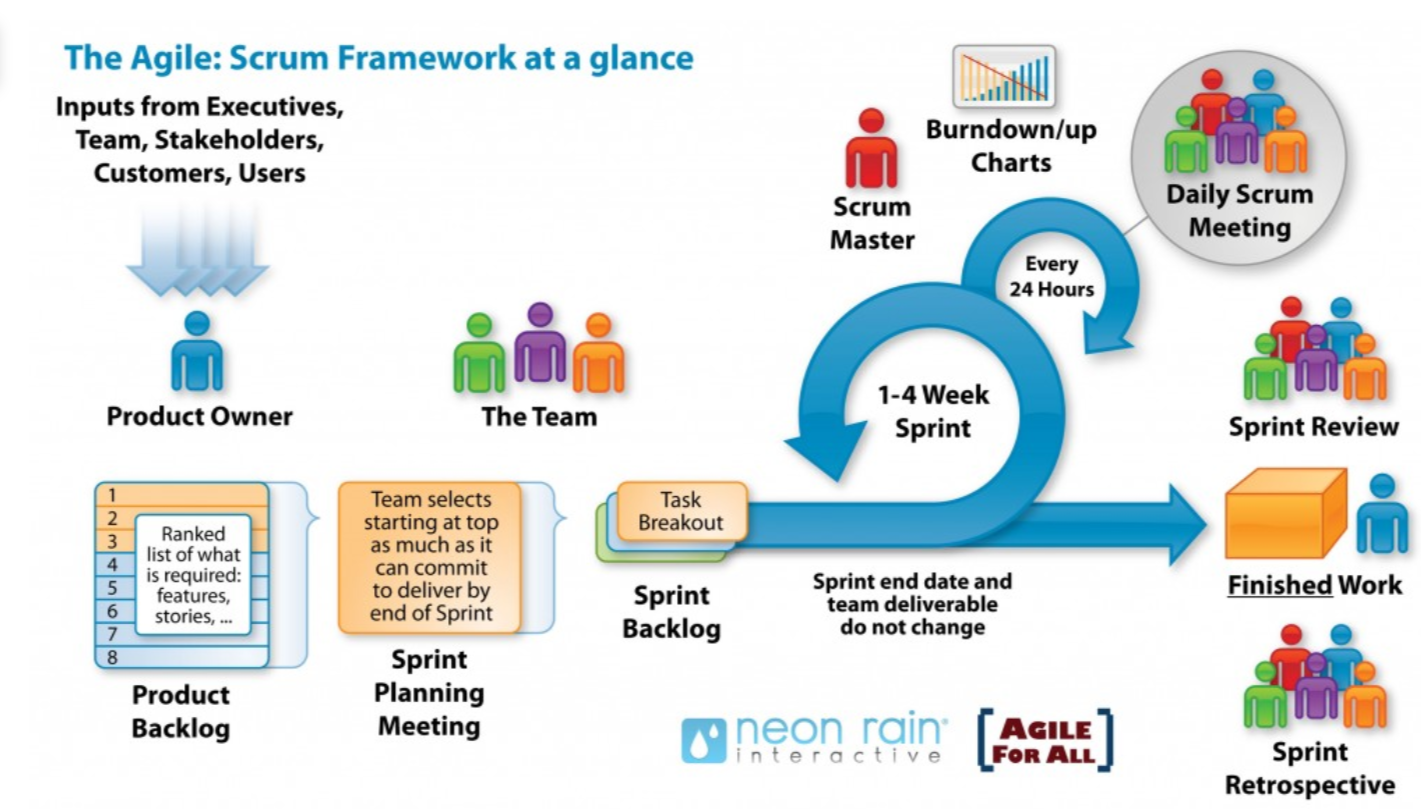
\includegraphics[width=0.95\textwidth]{sprint.png}
        \end{center}
    \end{frame}

    \subsection{ScrumBut}

    \begin{frame}
        \frametitle{ScrumBut}
        \begin{itemize}
            \item Персонализация задач/багов
            \begin{itemize}
                \item ``Твой баг, ты и правь''
                \item ``Маша --- тестировщик, задачи на тестирование ей''
                \item Распределение задач в начале спринта
            \end{itemize}
            \item Водопад внутри спринта
            \item Ориентация на тулы вместо прямой коммуникации
            \item 6-12-недельные спринты, перерывы между спринтами
            \item Big Design Up-Front (BDUF)
            \item Отсутствие Scrum master’а
            \item Демо по принципу ``Да мы ничего особого не сделали в этом спринте''
            \item Наличие тимлида
        \end{itemize}
    \end{frame}

    \begin{frame}
        \frametitle{Когда Scrum может работать плохо}
        \begin{itemize}
            \item Fixed-cost/fixed-time проекты
            \item Безответственные, низко мотивированные работники
            \item Слишком узкоспециализированные работники
            \item Неполноставочники
            \item Большое количество внешних зависимостей
            \item Legacy или системы повышенной надёжности
            \item Распределённые команды 
            \begin{itemize}
                \item За последний год все научились работать удалённо уже
            \end{itemize}
        \end{itemize}
    \end{frame}

    \begin{frame}
        \frametitle{Заключение}
        \begin{center}
            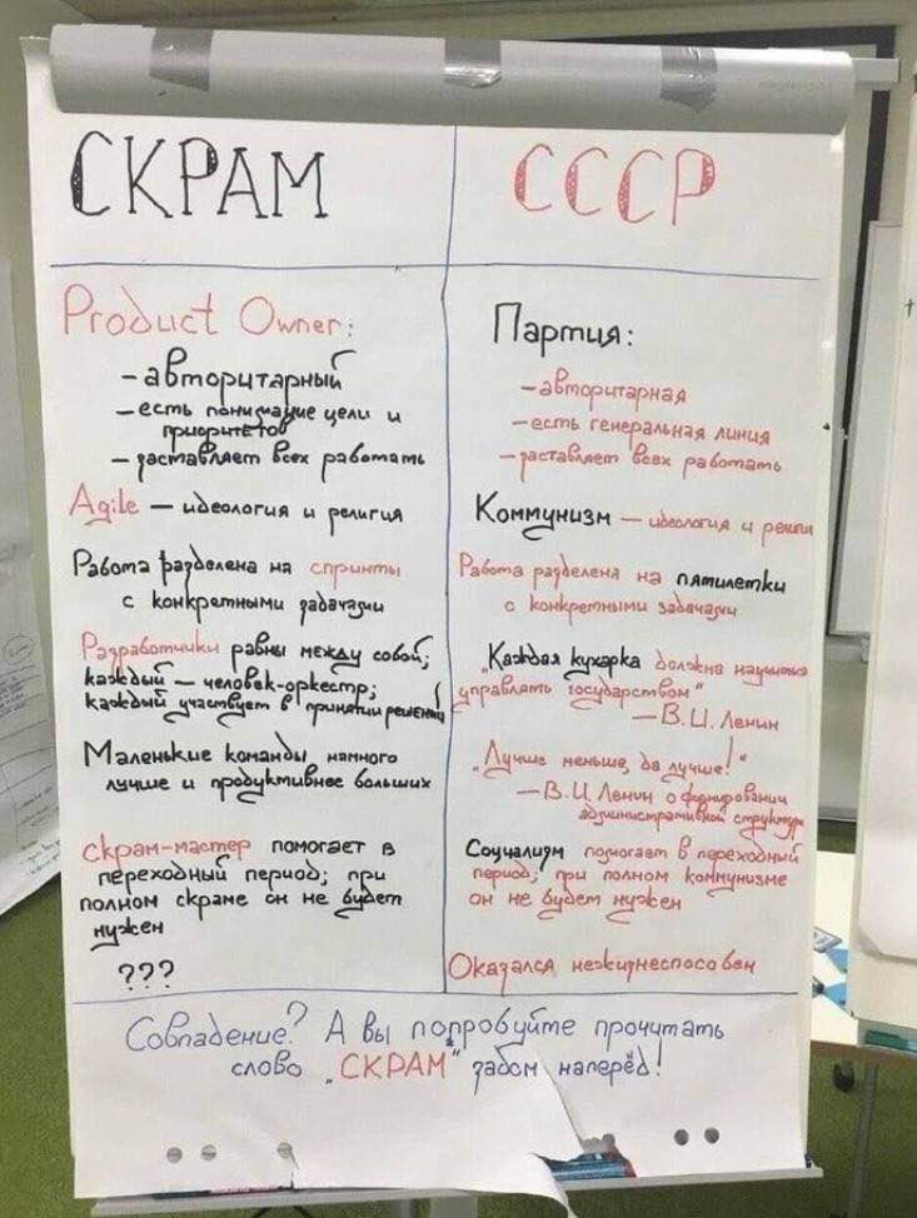
\includegraphics[width=0.45\textwidth]{soviet-union.png}
        \end{center}
    \end{frame}

\end{document}